\chapter{Algorytm animacji awatara}
\label{cha:implementacja}
Jak wspomniano we wcześniejszych rozdziałach, działanie algorytmu zaimplementowanego na potrzeby tej pracy inżynierskiej można podzielić na kilka kluczowych etapów. Poniższy rozdział zawiera szczegółowy opis każdego z nich. Zostaną także zaprezentowane efekty otrzymane w konkretnych krokach.

\section{Struktura programu}
Do stworzenia algorytmu wykorzystano język programowania Python umożliwiający tworzenie różnego rodzaju funkcji. Zostały one zaimplementowane dla każdego istotnego etapu programu, które zostały przedstawione na poniższym schemacie (Rys. \ref{fig:algorithmStructure}).

\begin{figure}[h]
	\centering
	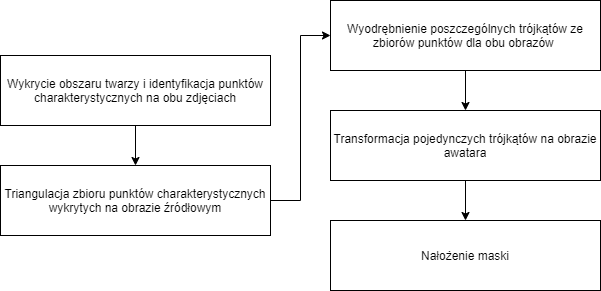
\includegraphics[width=14cm]{zdjęcia/struktura.png}
	\caption{Etapy algorytmu animacji awatara.} 
	\label{fig:algorithmStructure}
\end{figure}

Kluczową kwestią jest wcześniejsze wczytanie danych, czyli obrazu źródłowego, przez który rozumie się zdjęcie mające posłużć jako baza do przekształcenia awatara oraz jego obraz, na którym nastąpi animacja.

% \begin{itemize}
%     \item Wykrycie obszaru twarzy i identyfikacja punktów charakterystycznych na obydwu zdjęciach
%     \item Triangulacja zbioru punktów charakterystycznych wykrytych na obrazie źródłowym
%     \item Wyodrębnienie odpowiadających sobie sympleksów ze zbiorów punktów 
%     \item Transformacja pojedynczych trójkątów
%     \item Nałożenie maski 
% \end{itemize}

\section{Wykrycie twarzy oraz punktów charakterystynczych}
Pierwszym krokiem jest wykrycie obszaru twarzy oraz identyfikacja jej punktów charakterystycznych. Zostało to zrealizowane z użyciem gotowych funkcji udostępnianych przez bibliotekę dlib:
\begin{itemize}
    \item get\_frontal\_face\_detector() - funkcja nie przyjmuje żadnych parametrów, zwraca wytrenowany obiekt umożliwiający detekcję twarzy. Model został wytrenowany przy pomocy algorytmu działającego w oparciu o klasyfikator SVM i deskryptor HOG, opisany w podrozdziale \ref{sec:svmhog}. 
    \item shape\_predictor() - parametrem wejściowym jest wytrenowany model umożliwiający poprawną lokalizację punktów charakterystycznych. Został on wyszkolony na podstawie algorytmu przedstawionego w podrozdziale \ref{sec:landmarks}. Wynikiem zastosowania danej funkcji jest obiekt, który generuje owy zestaw punktów zlokalizowanych na obrazie przekazanym jako dane wejściowe.
\end{itemize}

\begin{figure}[h]
	\centering
	\begin{subfigure}{0.35\textwidth}
		\centering
		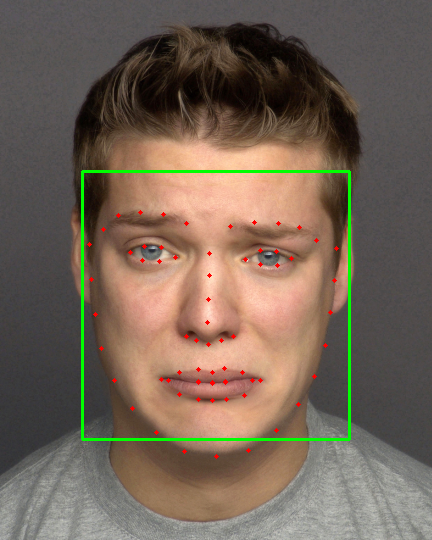
\includegraphics[height=5.5cm]{zdjęcia/detected_landmarks_src.png}
		\subcaption{\label{detected_landmarks_src}}
	\end{subfigure}
	\begin{subfigure}{0.35\textwidth}
		\centering
		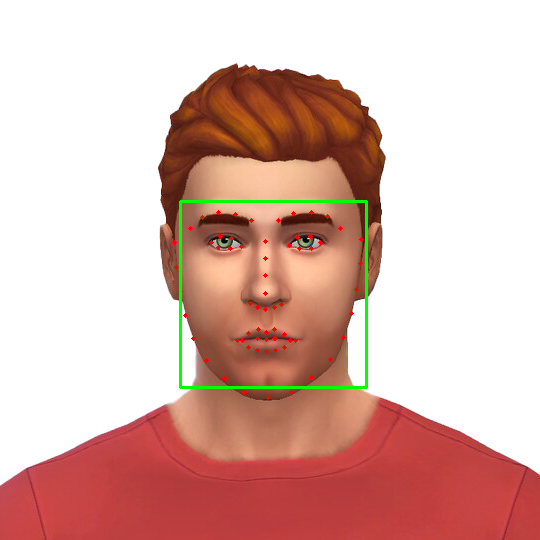
\includegraphics[height=5.5cm]{zdjęcia/detected_landmarks_avatar.png}
		\subcaption{\label{detected_landmarks_avatar}}
	\end{subfigure}
	
	\caption{\label{fig:detectedLandmarks}Twarz i punkty wykryte na obrazie źródłowym \protect\subref{detected_landmarks_src} oraz na awatarze \protect\subref{detected_landmarks_avatar}.}
\end{figure}

Wybrane funkcje zdają się być wystarczające do osiągnięcia zamierzonego rezultatu. Można założyć, iż przetwarzane obrazy zawierają dobrze widoczny obszar twarzy ustawionej w pozycji frontowej. Z tego powodu dokładność działania narzędzia wykrywającego twarz oraz punkty charakterystyczne jest wysoka.


\begin{minted}
[
frame=lines,
label=Wykrycie twarzy oraz punktów charakterystycznych,
framesep=2mm,
baselinestretch=1.2,
breaklines,
bgcolor=white,
fontsize=\footnotesize,
linenos
]
{python}
def detect_face_and_landmarks(img):
    detector = dlib.get_frontal_face_detector()
    predictor = dlib.shape_predictor('./data/shape_predictor_68_face_landmarks.dat')

    gray = cv2.cvtColor(imutils.resize(img), cv2.COLOR_BGR2GRAY)
    rects = detector(gray, 1)
    facial_landmarks = []

    if rects:
        for rect in rects:
            facial_landmarks = predictor(gray, rect)
            facial_landmarks = face_utils.shape_to_np(facial_landmarks)

    return img, facial_landmarks
\end{minted}

Efektem wizualnym użycia powyższej funkcji są obrazy przedstawione na Rys.\ref{fig:detectedLandmarks}. Na każdym ze zdjęć została zlokalizowana twarz, którą zaznaczono zielonym prostokątem oraz jej kluczowe elementy, w postaci 68 punktów oznaczonych kolorem czerwonym. W następnych etapach posłużą one jako baza, na której będą wykonywane wszelkie operacje. 

% \inputminted[firstline=2, lastline=12]{octave}{BitXorMatrix.m}
\section{Triangulacja zbioru punktów}
Kolejnym etapem działania algorytmu animacji awatara jest triangulacja zbioru punktów charakterystycznych, zlokalizowanych na obszarze twarzy obrazu źródłowego. Celem jej zastosowania jest podział przestrzeni na nieskomplikowane trójkąty posiadające ostre kąty, co zapewni przejrzystość i równomierność figur.

W bibliotece OpenCV dostępne są funkcje, generujące triangulację Delone dla zestawu punktów. Ich użycie jest bardzo proste i intuicyjne. Z wykorzystaniem modułu Subdiv2D( Rect rect ), dla którego parametrem wejściowym jest prostokątny obszar obejmujący wszystkie istotne punkty, zostaje wygenerowany pusty obiekt. Następnie za pomocą funkcji insert() można dodać do niego listę elementów charakterystycznych, dla których chcemy dokonać triangulacji. Ostatnim krokiem jest wywołanie funkcji getTriangleList(), która zwraca listę trójkątów wygenerowanych przez algorytm. 

\begin{minted}
[
frame=lines,
label=Triangulacja Delone dla zbioru punktów,
framesep=2mm,
baselinestretch=1.2,
breaklines,
bgcolor=white,
fontsize=\footnotesize,
linenos
]
{python}
def delaunay_triangulation(src_points, avatar_points):
    points_list = list(src_points)
    delaunay_subdivision = cv2.Subdiv2D((*src_points.min(axis=0), *src_points.max(axis=0)))
    delaunay_subdivision.insert(points_list)

    for x1, y1, x2, y2, x3, y3 in delaunay_subdivision.getTriangleList():
        indexes_set = [(src_points == single_point).all(axis=1).nonzero()[0][0]
                       for single_point in [[x1, y1], [x2, y2], [x3, y3]]]

        src_triangles = generate_xy_for_indexes(src_points, indexes_set)
        avatar_triangles = generate_xy_for_indexes(avatar_points, indexes_set)
        yield [np.array(src_triangles), np.array(avatar_triangles)]
        

def generate_xy_for_indexes(points, indexes):
    return [points[single_index] for single_index in indexes]
\end{minted}

Funkcja zaimplementowana w celu rozwiązania tej części problemu generuje opisaną powyżej triangulację. Kolejną istotną kwestią jest wyodrębnienie analogicznych trójkątów z obydwu list punktów. Moduł getTriangleList() zwraca współrzędne wszystkich wierzchołków każdego z wygenerowanych trójkątów. W prosty sposób można odnaleźć ich indeksy w zbiorze punktów charakterystycznych obrazu źródłowego, a następnie zidentyfikować analogiczne elementy w zbiorze punktów wygenerowanych z obrazu awatara.

\begin{figure}[h]
	\centering
	\begin{subfigure}{0.35\textwidth}
		\centering
		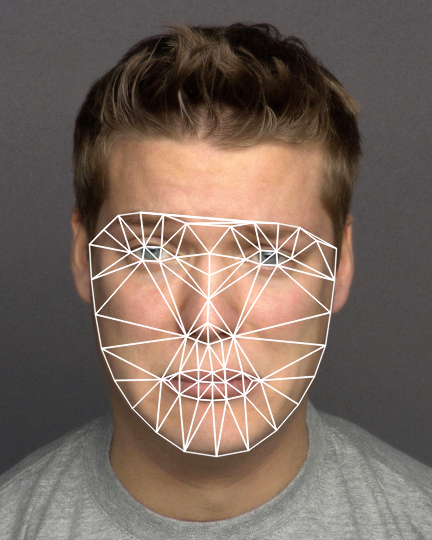
\includegraphics[height=5.5cm]{zdjęcia/triangulation_src.png}
		\subcaption{\label{triangulation_src}}
	\end{subfigure}
	\begin{subfigure}{0.35\textwidth}
		\centering
		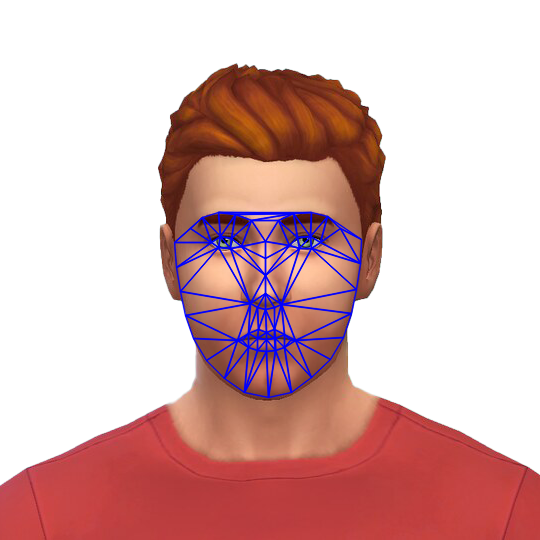
\includegraphics[height=5.5cm]{zdjęcia/triangulation_avatar.png}
		\subcaption{\label{triangulation_avatar}}
	\end{subfigure}
	
	\caption{\label{fig:triangulation}Triangulacja punktów char. obrazu źródłowego \protect\subref{triangulation_src} oraz awatara \protect\subref{triangulation_avatar}.}
\end{figure}

Na Rys. \ref{fig:triangulation} można zaobserwować efekt działania tej części programu. Na pierwszym obrazie zaznaczono trójkąty otrzymane w wyniku zastosowania triangulacji, natomiast na drugim zaznaczono analogiczne trójkąty.




\section{Transformacja trójkątów}
No to tutaj jak to się odbywa, czyli dłuższa sprawa w sumie. Trzeba dać kod, może nie cały plus jakieś zdjęcia, że trójkąty awatara modyfikowane do trójkątów z src, a potem sklejane w maskę. 
tutaj kolejna funkcja, czyli czysta transformacja poprzez te funkcje warp itd itp
\begin{minted}
[
frame=lines,
framesep=2mm,
baselinestretch=1.2,
breaklines,
bgcolor=white,
fontsize=\footnotesize,
linenos
]
{python}
def animate_avatar(avatar_img, avatar_points, src_img, src_points):
    new_avatar_face = np.zeros(src_img.shape, np.uint8)

    for src_triangle_points, avatar_triangle_points in delaunay_triangulation(src_points, avatar_points):
        avatar_img_cropped, avatar_triangle, _ = crop_single_triangle(avatar_triangle_points, avatar_img)
        src_img_cropped, src_triangle, b_rect = crop_single_triangle(src_triangle_points, src_img)

        warped_triangle = transform_triangle(avatar_triangle, avatar_img_cropped, src_triangle, src_img_cropped)
        add_triangle_to_new_face_area(new_avatar_face, warped_triangle, b_rect)

    return generate_new_face(avatar_img, avatar_points, new_avatar_face, src_points)


def crop_single_triangle(single_triangle, img):
    b_rect = cv2.boundingRect(single_triangle)
    triangle_img = [(indexes[0] - b_rect[0], indexes[1] - b_rect[1]) for indexes in single_triangle]
    cropped_img = img[b_rect[1]:b_rect[1] + b_rect[3], b_rect[0]:b_rect[0] + b_rect[2]]

    return cropped_img, triangle_img, b_rect


def transform_triangle(avatar_triangle, avatar_img_cropped, src_triangle, src_img_cropped):
    transform_matrix = cv2.getAffineTransform(np.float32(avatar_triangle), np.float32(src_triangle))

    warped_triangle = cv2.warpAffine(avatar_img_cropped, transform_matrix,
                                     (src_img_cropped.shape[1], src_img_cropped.shape[0]), None,
                                     flags=cv2.INTER_LINEAR, borderMode=cv2.BORDER_REFLECT_101)

    mask = np.zeros(src_img_cropped.shape, dtype=np.uint8)
    mask = cv2.fillConvexPoly(mask, np.int32(src_triangle), (1.0, 1.0, 1.0), 16, 0)
    warped_triangle *= mask

    return warped_triangle


def add_triangle_to_new_face_area(new_face, warped_triangle, b_rect):
    (x, y, w, h) = b_rect
    new_face_gray = cv2.cvtColor(new_face[y: y + h, x: x + w], cv2.COLOR_BGR2GRAY)
    _, mask = cv2.threshold(new_face_gray, 0, 255, cv2.THRESH_BINARY_INV)
    warped_triangle = cv2.bitwise_and(warped_triangle, warped_triangle, mask=mask)

    new_face[y: y + h, x: x + w] += warped_triangle
\end{minted}

\section{Nałożenie maski}

\begin{minted}
[
frame=lines,
framesep=2mm,
baselinestretch=1.2,
breaklines,
bgcolor=white,
fontsize=\footnotesize,
linenos
]
{python}
def generate_new_face(avatar_img, avatar_points, new_avatar_face, src_points):
    transform = PiecewiseAffineTransform()
    transform.estimate(choose_specific_points(avatar_points), choose_specific_points(src_points))

    face = warp(new_avatar_face, transform, output_shape=avatar_img.shape, order=0, mode='wrap')
    face = cv2.normalize(face, None, 0, 255, cv2.NORM_MINMAX, cv2.CV_8U)

    face_gray = cv2.cvtColor(face, cv2.COLOR_BGR2GRAY)
    _, mask = cv2.threshold(face_gray, 0, 255, cv2.THRESH_BINARY_INV)
    new_avatar_img = cv2.bitwise_and(avatar_img, avatar_img, mask=mask)

    new_avatar_img += face

    return new_avatar_img
\end{minted}

No to jak wygląda maska przed rozciągnięciem, a jak po, plus ta funkcja która tam za to odpowiada. W sumie tą funkcję choose można tylko opisać, tutaj pasuje też załączyć zdjęcie z zaznaczonymi 

\begin{figure}[h]
	\centering
	\begin{subfigure}{0.35\textwidth}
		\centering
		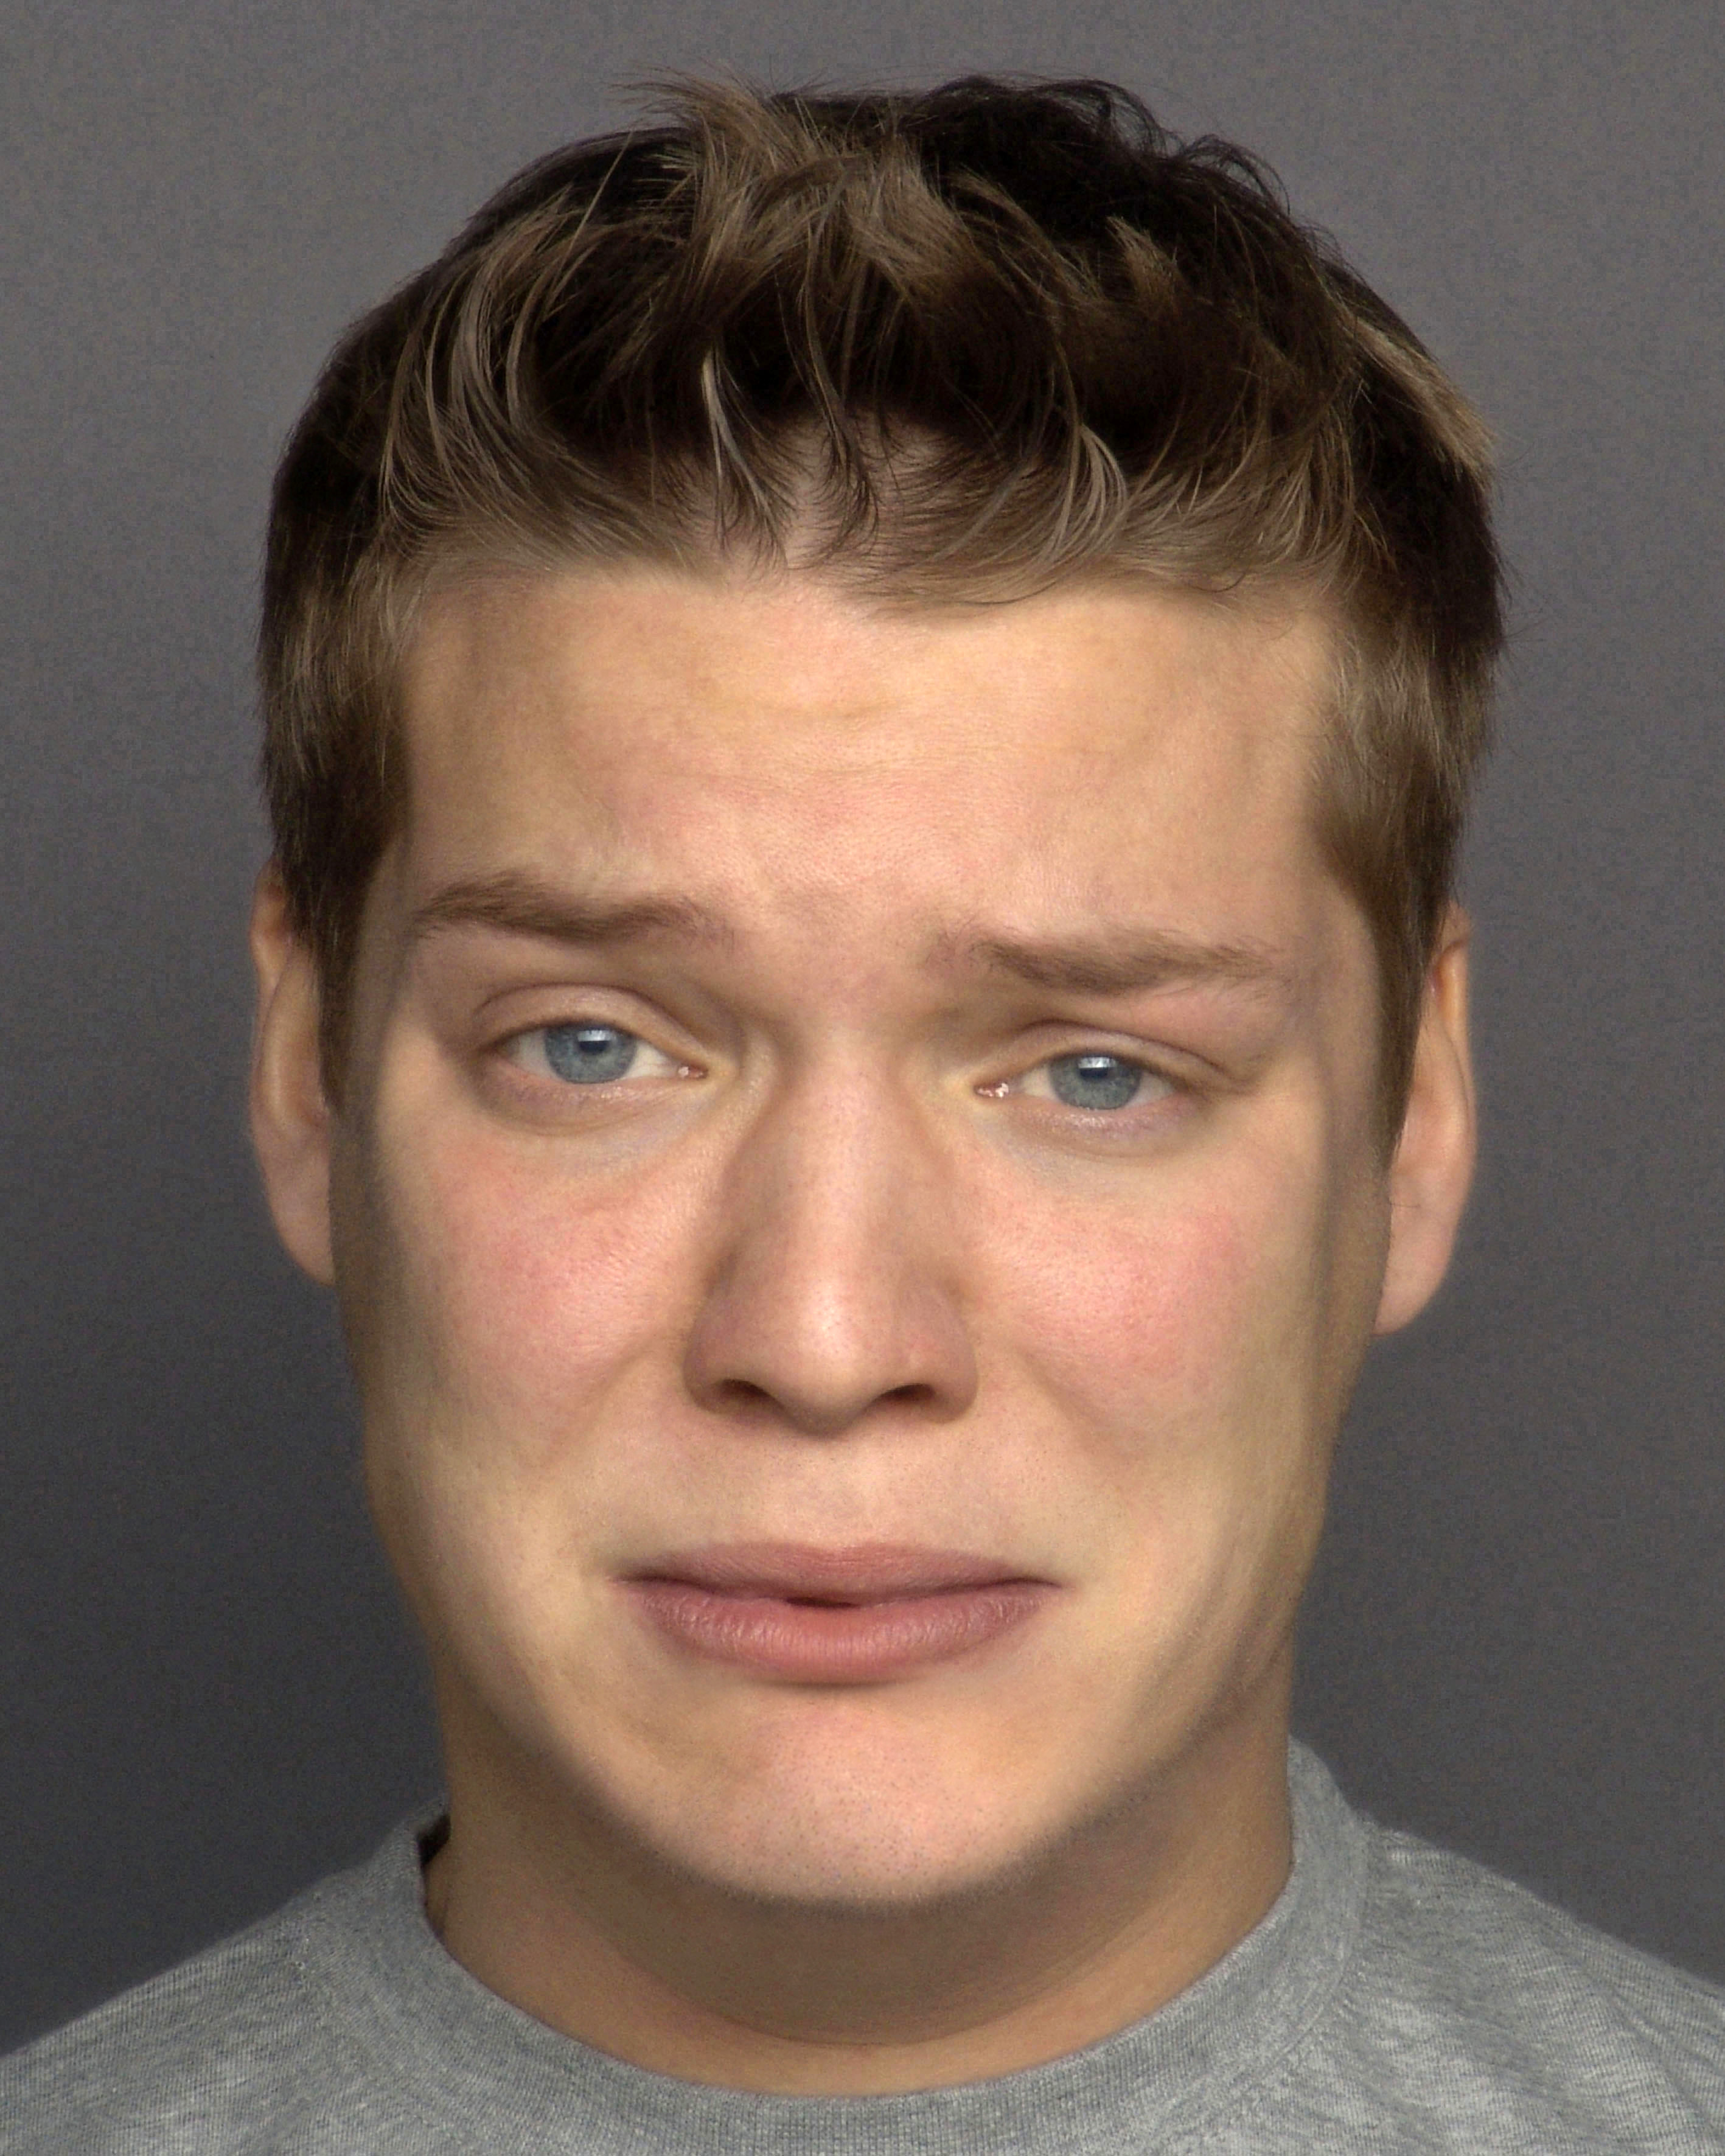
\includegraphics[height=5.5cm]{zdjęcia/src_img.jpg}
		\subcaption{\label{src_img}}
	\end{subfigure}
	\begin{subfigure}{0.35\textwidth}
		\centering
		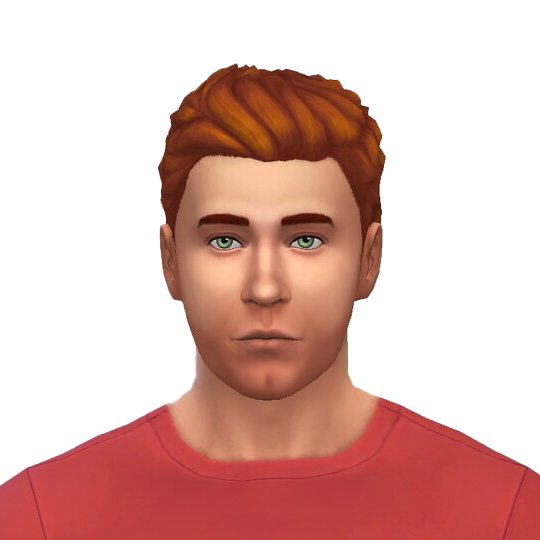
\includegraphics[height=5.5cm]{zdjęcia/avatar.png}
		\subcaption{\label{avatar}}
	\end{subfigure}
	\begin{subfigure}{0.35\textwidth}
		\centering
		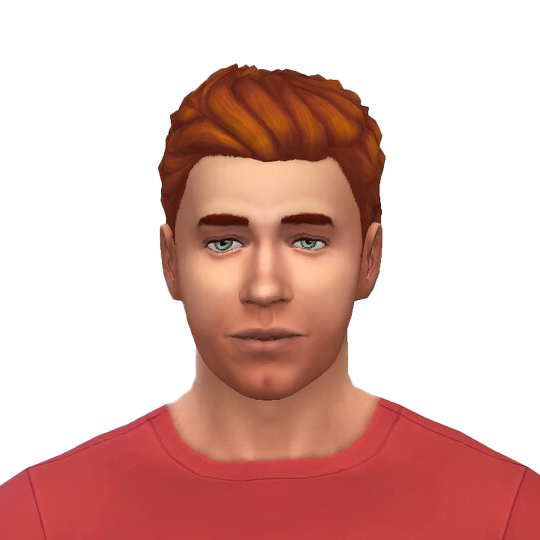
\includegraphics[height=5.5cm]{zdjęcia/result_avatar.png}
		\subcaption{\label{result_avatar}}
	\end{subfigure}
	
	\caption{\label{fig:result}Rezultat działania algorytmu animacji awatara \protect\subref{result_avatar} na zdjęciu źródłowym \protect\subref{src_img} oraz awatarze \protect\subref{avatar}.}
\end{figure}



